\chapter*{Sortie de préparation Toulouse – Figeac\markboth{Sortie de préparation Toulouse – Figeac}{}}
\section*{11 novembre 2014}
Première sortie test ce week end. J'ai profité du pont du 11 novembre pour partir avec le vélo, en configuration voyage, direction Figeac.

 L'itinéraire prévu fait environ 200km, faisable sur 2 ou 3 jours, selon le nombre de km que j'arriverai à faire sur une journée.

 Départ dimanche matin à 9h, la pesée de départ vélo chargé avec les affaires, la nourriture pour 3 jours et 3.5L d'eau me donne 41.5kg :
\begin{center} 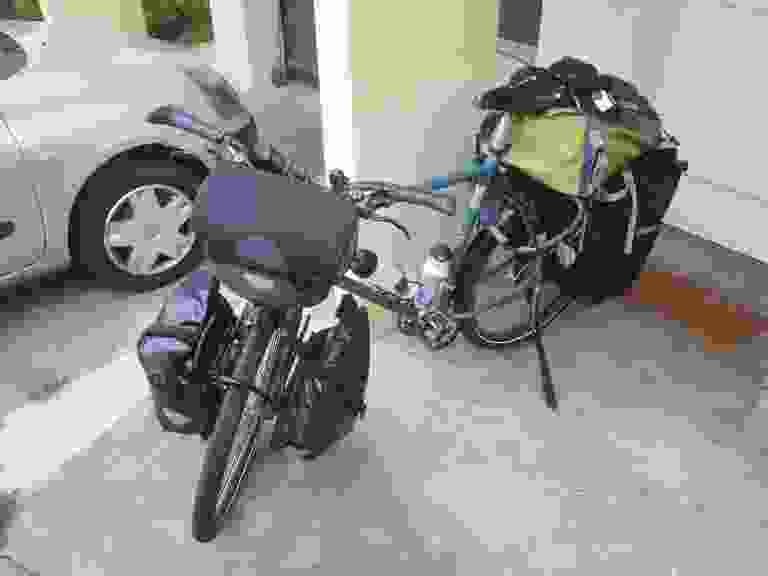
\includegraphics[width=\mywidth]{../wp-content/uploads/2014/11/PB092254.jpg} \end{center}

 Quelques tours de roue dans la rue, et c'est un faux départ car les vitesses que j'avais pourtant bien réglées quelques jours avant ne passent pas bien, ainsi que le frein arrière qui est un peu mou. Retour à la maison pour modifier les réglages. En fait, c'est la sacoche de guidon, en appuyant sur les câbles, qui a déréglée les vitesses.

 Deuxième départ à 10h, cette fois c'est le bon !
Début de l'itinéraire sur le canal latéral direction Bordeaux, 50km de plat pour commencer.
\begin{center} 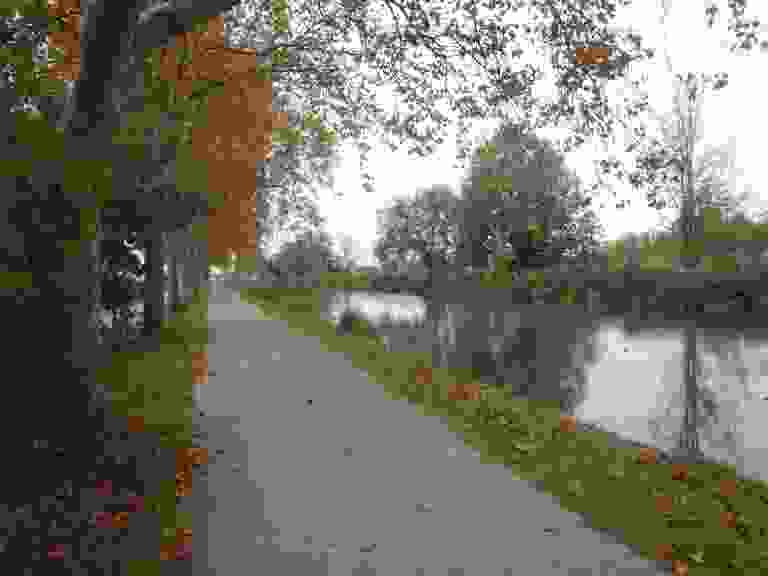
\includegraphics[width=\mywidth]{../wp-content/uploads/2014/11/PB092259.jpg} \end{center}

 Au bout d'une vingtaine de km, la pluie arrive, fine mais régulière.
\begin{center} 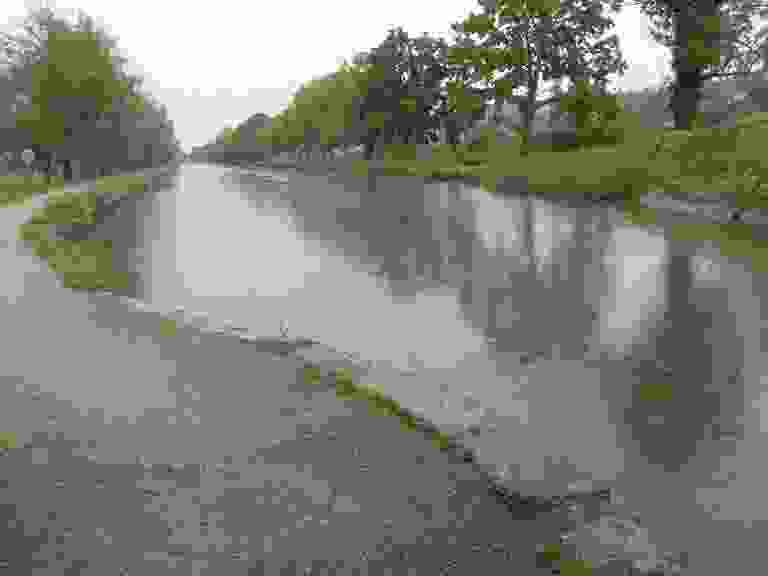
\includegraphics[width=\mywidth]{../wp-content/uploads/2014/11/PB092260.jpg} \end{center}

 J'enfile mes protections de jambes, que je n'ai pas encore testées. Elles sont légères mais plutôt minimalistes, je sais pas ce que ça va donner.
\begin{center} 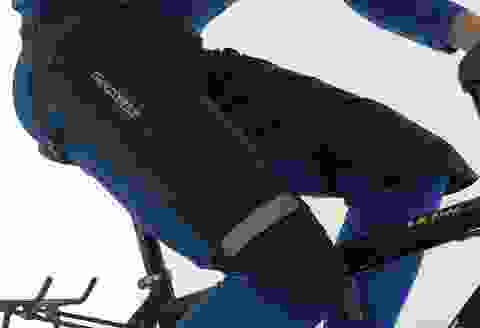
\includegraphics[width=\mywidth]{../wp-content/uploads/2014/11/rainlegs02.jpg} \end{center}

Finalement, sous une pluie fine, ininterrompue pendant 3 ou 4h, c'était parfait, la protection jusqu'au genou est suffisante pour avoir les jambes au sec. Il faut juste ne pas oublier d'essuyer la selle quand on remonte sur le vélo après une pause !

 Au bout de 50km, je quitte le canal au niveau de Saint Porquier.
\begin{center} 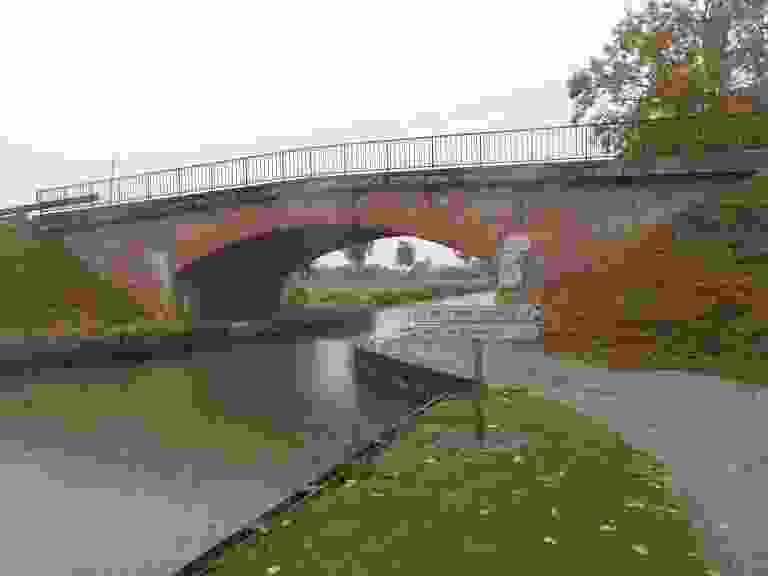
\includegraphics[width=\mywidth]{../wp-content/uploads/2014/11/PB092264.jpg} \end{center}
\begin{center} 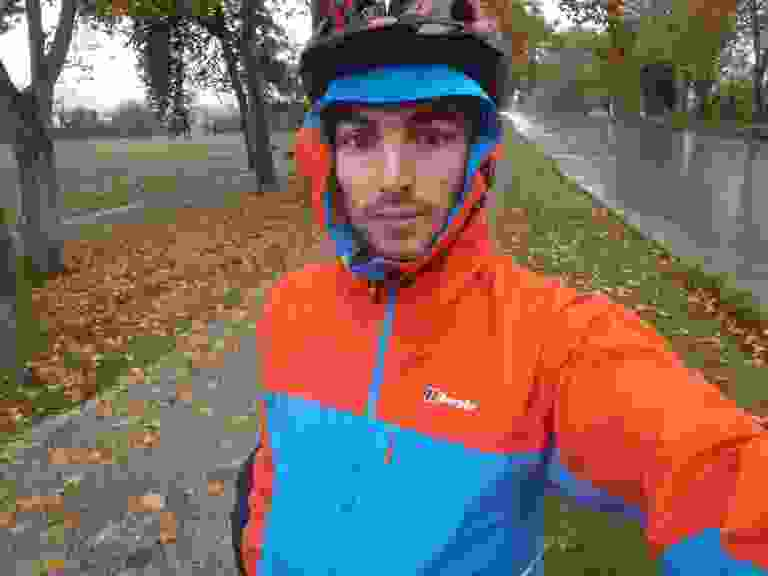
\includegraphics[width=\mywidth]{../wp-content/uploads/2014/11/PB092265.jpg} \end{center}

 Je continue en direction de Ville Dieu du Temple, où je m'arrête pour pique-niquer, à l'abri devant l'entrée de l'école du village.

 Passage par Lafrançaise, après une côte longue et bien raide. J'ai pu tester la petite vitesse du vélo, le 24-34 devrait me permettre de bien passer la plupart des côtes, à 4km/h, ça mouline sans trop d'effort.
 
\begin{center} 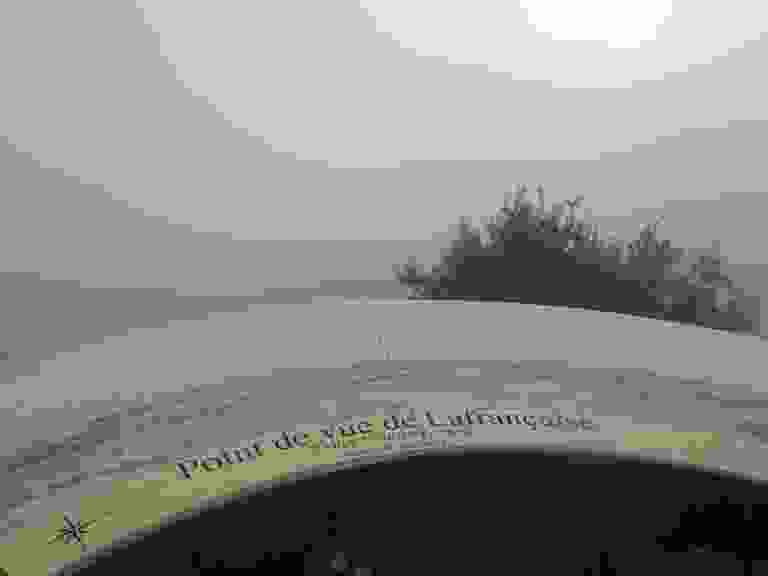
\includegraphics[width=\mywidth]{../wp-content/uploads/2014/11/PB092266.jpg} \end{center}

\pagebreak
 Après presque 90km, j'arrive au niveau de Castelnau Montratier. Il est 17h15, il va être temps de trouver un endroit pour le bivouac.
\begin{center} 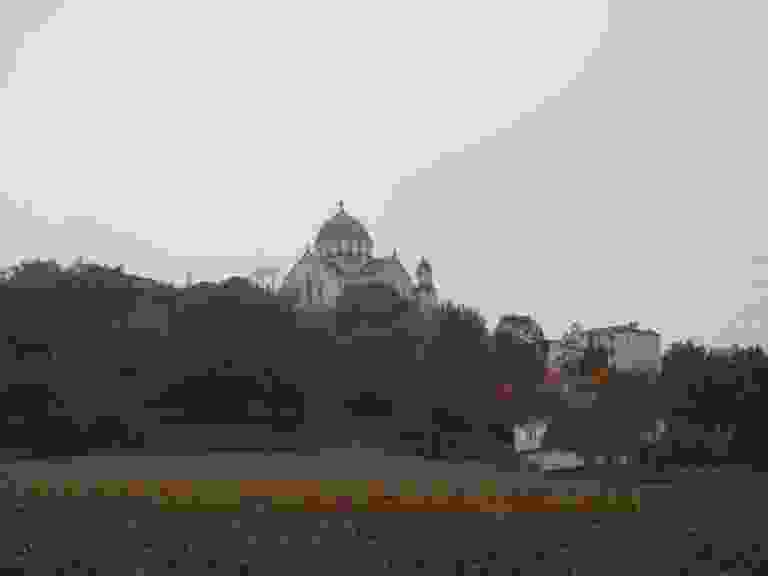
\includegraphics[width=\mywidth]{../wp-content/uploads/2014/11/PB092270.jpg} \end{center}

 Quelques km après la sortie du village, je vois un petit sentier qui monte au bord de la route et je décide d'aller voir ce qu'il y a en haut. Après une centaine de mètres, je tombe sur un emplacement idéal pour passer la nuit.
\begin{center} 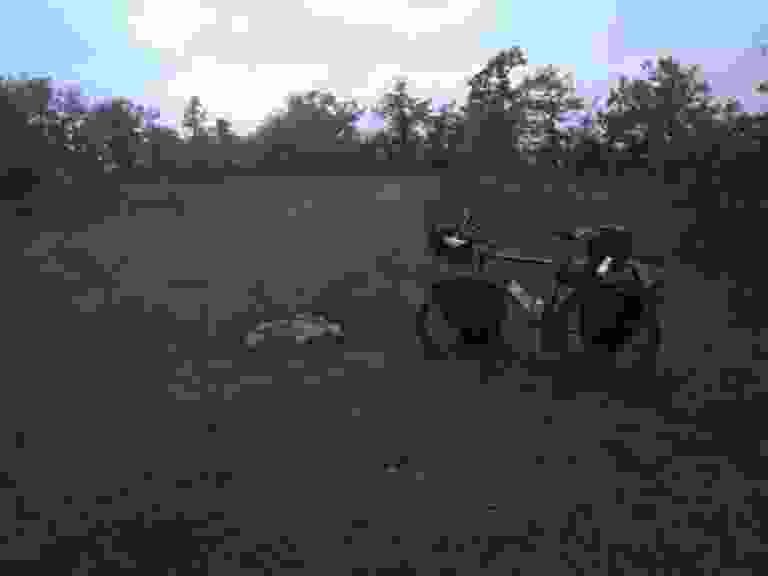
\includegraphics[width=\mywidth]{../wp-content/uploads/2014/11/PB092273.jpg} \end{center}

 J'installe la tente alors que la nuit commence à tomber et heureusement la pluie s'était arrêtée quelques heures avant. 
\begin{center} 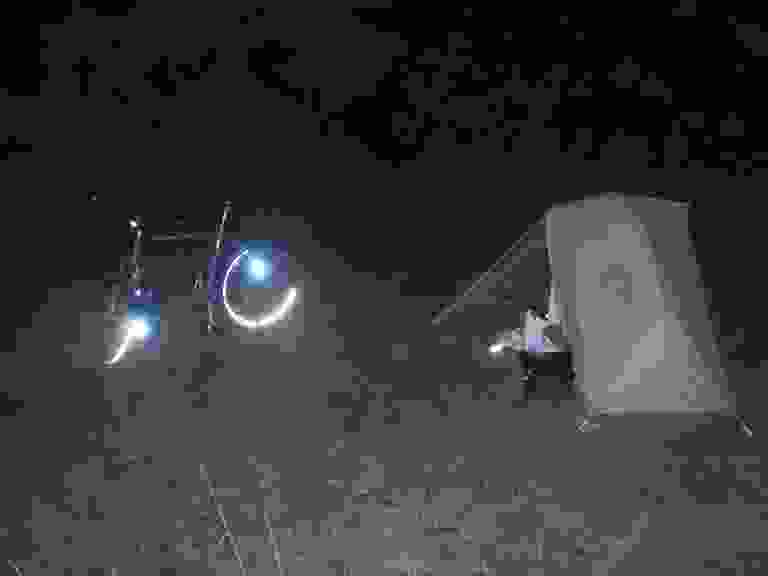
\includegraphics[width=\mywidthreduced]{../wp-content/uploads/2014/11/PB092274.jpg} \end{center}

 Le lendemain matin, départ un peu avant 9h en direction de Cahors. Au bout d'environ 15km, je croise la route nationale et je m'aperçois que je n'ai pas pris la bonne route, j'avais raté une bifurcation la veille juste avant de m'arrêter.
 Du coup, pour éviter de rouler sur la nationale, je décide de changer d'itinéraire et de continuer direction Lalbenque, pour ensuite rejoindre la vallée du Célé au niveau de Saint Cirq Lapopie.
\begin{center} 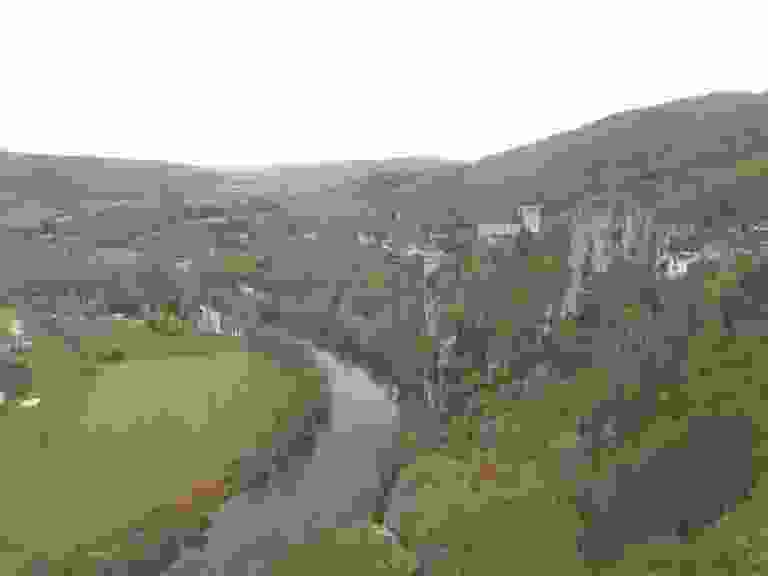
\includegraphics[width=\mywidthreduced]{../wp-content/uploads/2014/11/PB102280.jpg} \end{center}

J'arrive à Saint Cirq Lapopie vers 11h30, par le haut du village.

\begin{center} 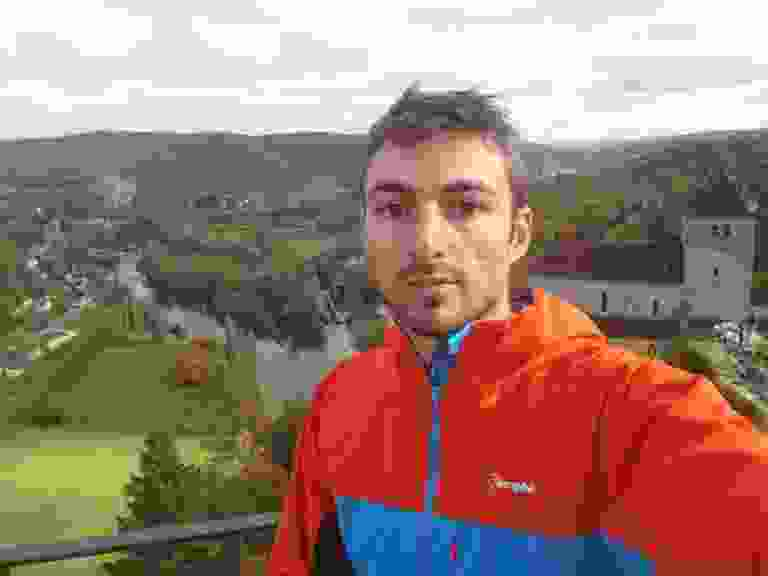
\includegraphics[width=\mywidth]{../wp-content/uploads/2014/11/PB102288.jpg} \end{center}

 J'en profite pour visiter rapidement le plus beau village de France 2012.
 
\begin{center} 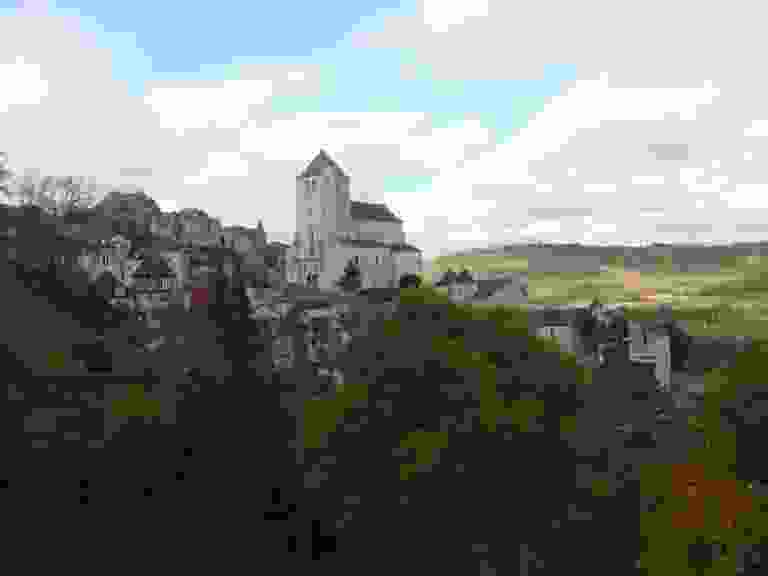
\includegraphics[width=\mywidth]{../wp-content/uploads/2014/11/PB102289.jpg} \end{center}

\pagebreak
 Je descend au bord du Lot en dessous de Saint Cirq Lapopie, afin de rejoindre la vallée du Célé, direction Figeac.
\begin{center} 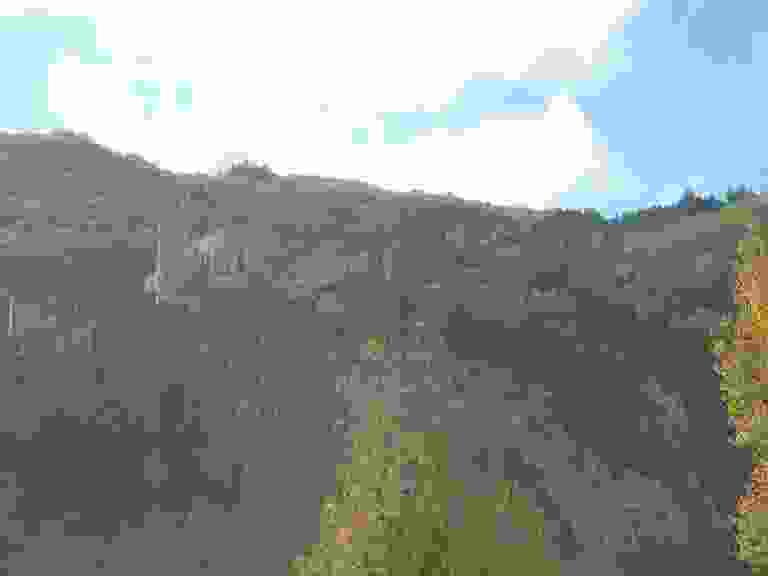
\includegraphics[width=\mywidth]{../wp-content/uploads/2014/11/PB102291.jpg} \end{center}

 Encore quelques km, avant de m'arrêter vers 13h pour pique-niquer au bord de la rivière, au niveau de Sauliac-sur-Célé.
\begin{center} 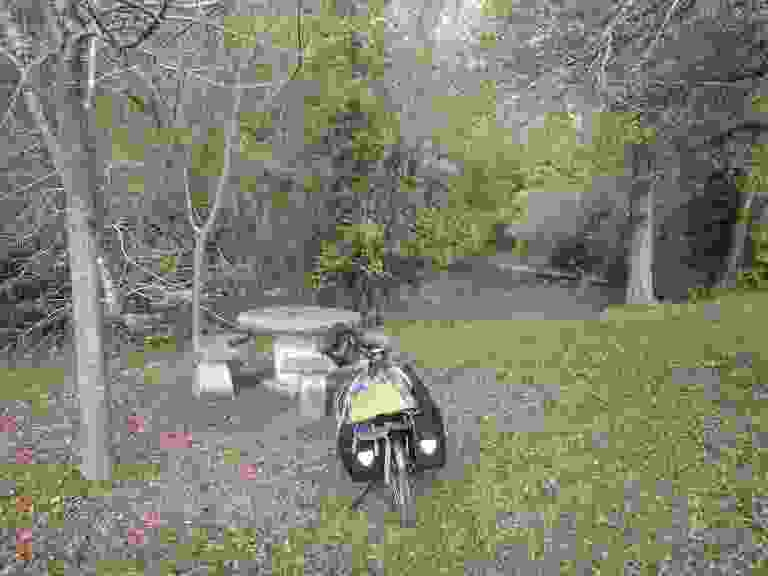
\includegraphics[width=\mywidth]{../wp-content/uploads/2014/11/PB102292.jpg} \end{center}

 Il me reste une quarantaine de km le long de la rivière pour rejoindre Figeac.
 
 Je profite du passage à Espagnac Saint Eulalie pour aller jeter un œil à l'ancien prieuré.
\begin{center} 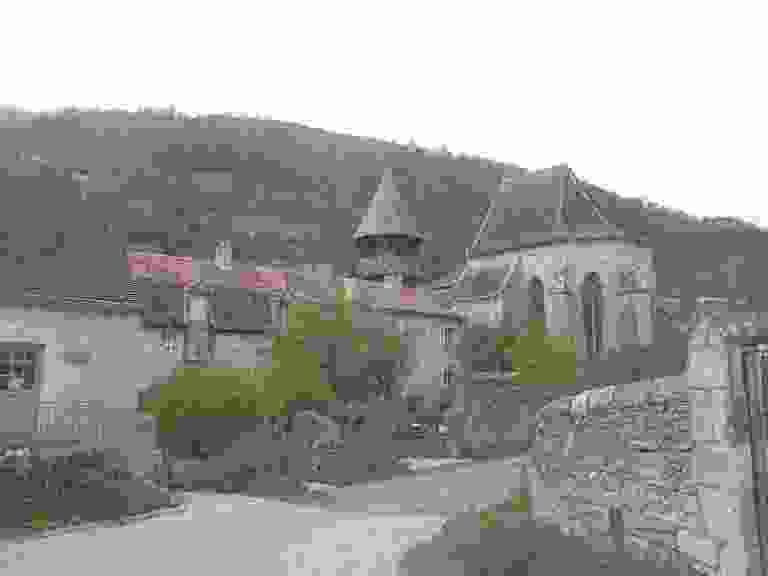
\includegraphics[width=\mywidth]{../wp-content/uploads/2014/11/PB102295.jpg} \end{center}

 J'arrive finalement à Figeac vers 17h, avec 104km dans les jambes.
 
\subsection*{Bilan de la sortie}

 Au niveau du vélo, je suis plutôt rassuré, j'ai de bonnes sensations et une position satisfaisante. Les réglages de vitesses seront à peaufiner car le petit plateau a du mal à passer, peut être qu'un changement de dérailleur avant sera nécessaire.

 Au niveau de la vitesse, je m'aperçois que je ne peux pas rouler très vite. J'ai fait les deux jours à 16km/h de moyenne, sur un parcours vallonné par endroit. Mais même sur les portions plates comme le canal, la moyenne ne dépasse pas 18km/h. Sur les 2 jours, les sensations ont été globalement les mêmes : mise en route le matin assez difficile, un peu de temps pour trouver le rythme. Puis, bonnes sensations en fin de matinée, ça avance bien. Enfin, après-midi plus laborieuse, la vitesse moyenne chute, la fatigue se fait sentir.

 Au niveau de l'endurance, je me rend compte que sur un parcours comme celui-là, il est faisable de faire 100km/jour, mais ça reste une grosse journée, sans trop de pause. Est-ce que l'enchainement de telles distance sur plusieurs jours sera possible ?

 Pour le physique, ça s'est bien passé, pas de douleur particulière à signaler. J'ai roulé la première journée sans cuissard, mais j'ai quand même dû le mettre pour le 2e jour, la selle cuir doit encore avoir besoin d'être rodée avant d'être grand confort comme je l'ai lu un peu partout.

 Concernant le bivouac, je suis très satisfait de la nouvelle tente, légère, simple à monter et pratique. J'avais aussi un nouveau matelas gonflable, un oreiller gonflable et un drap de couchage Thermolite. J'ai passé une bonne nuit, sans avoir froid. C'est plutôt positif car en général, les premières nuits sous tente ne sont pas les meilleures. Enfin, pour un premier camping sauvage seul, j'avais trouvé un bon emplacement pour camper à l'écart de la route, du coup, je n'ai pas été dérangé et ça s'est bien passé.

 Au final, j'ai bien apprécié la sortie. Même les passages sous la pluie sont bien passés. Cependant, pas de rencontre à signaler sur 2 jours, peut-être que la saison et la météo n'étaient pas propices. 
